\section {Offline Sketch Discovery}\label{sec:offline}
In the offline scenario, the input is a set of events
of all subjects and the output is a $k$-sketch 
for each subject $s$, denoted by $SK_s$. 
The sketch discovery process consists of two 
major steps: first generating the candidate themes of each subject (i.e., $\mathbb{N}_s$), 
and then discovering the sketches among those candidate themes. 

\subsection{Candidate Theme Generation}
Generating candidate themes for each subject is computationally 
expensive. In order to retain the candidate themes with rank no greater than $p$,
a brute-force approach needs to evaluate all the event windows with every possible length to generate accurate ranks. Since there could be $\mathbb{H}_s \choose 2$ event windows (with different lengths and ending sequence ids) associated with subject $s$, the total time complexity for the brute-force approach
is $O(\sum_{s \in S}|\mathbb{H}_s|^2)$. Such a complexity makes the solution infeasible even for moderate-sized datasets.

To improve the efficiency, 
we observe that it is not necessary to compute all the event windows to generate $\mathbb{N}_s$.
The intuition behind is that the upper bound value of event windows with longer lengths can be estimated from those
with shorter lengths. This means that we can compute event windows with increasingly lengths, and as the shorter event windows are computed, the longer event windows not in $\mathbb{N}_s$ can be pruned.
To realize such an intuition, we design the candidate generation algorithm
by adapting two novel window-based pruning methods which 
exploit the \emph{subadditivity} property among event windows with different window lengths.


\subsubsection{Overview of window pruning}
For each subject, its event windows can be grouped by window lengths. Our candidate
generation algorithm gradually evaluates a subject's event window from shorter
length to longer length. To support efficient pruning, 
we define two concepts, namely \emph{visiting-window bound} ($J_s$) and \emph{unseen-window bound} ($M_s$).
In particular, $J_s(w)$ is the upper bound of all the event windows about subject $s$ and with length $w$, i.e., $\forall w,J_s(w) \geq \max\{W_s(t,w).\overline{v} | t\in(0,w)\}$. 
$M_s(w)$ is the upper bound of all the event windows about subject $s$ with length larger than $w$, i.e., $M_s(w) \geq \max\{J_s(t) | t > w\}$.  These two bounds will be used for event window pruning and we will present how to estimate these two upper bounds in Sections~\ref{sec:visiting-window-bound} and~\ref{sec:useen-window-bound}.

%Utilizing these two bounds,
%we are able to design the \emph{visiting-window pruning} and \emph{useen-window pruning} techniques.

The overview of news theme generation algorithm is presented in Algorithm~\ref{algo:prune_overview}. We maintain two global structures $WI$ and $\beta$ (Lines~1-2). For each window length $w$, $WI(w)$ stores the top $p$ event windows with length $w$ among all the subjects and $\beta(w)$ is the $p$-th score among the candidates in $WI(w)$. 
In other words, $\beta(w)$ serves as a lower bound score. An event window with length $w$ is a candidate for the $k$-sketch only if its aggregate value is larger than $\beta(w)$. A priority queue $Q$ (Line 3) is used to provide an access order among the subjects. Each element in the queue is a triple $(s,w,q)$, where $s$ is a subject, $w$ indicates the next window length of $s$ to evaluate, and $q$ denotes the priority. We use the unseen-window bound (i.e., $M_s(w)$) as the priority during every iteration (Lines~13-14). Intuitively, an event window with higher $M_s(w)$ is more likely to spawn new event windows that can increase $\beta$ and benefit the subsequent pruning. During initialization, we insert, for each subject, an entry with window length $1$ and priority infinity into $Q$.

%the candidate with the maximum $M_s$ will be located on top of the priority queue. Intuitively, an event window with higher $M_s(w)$ is more likely to spawn new event windows that can increase the values in $\beta$ and facilitate the subsequent pruning. In the initialization step, we insert all the event windows with length $1$ into $Q$.

% and the comparison function in $Q$ is based on the value of $M_s$. C

%Instead of evaluating each subject one-by-one, we adapt a dynamic order of evaluation by using
%a priority queue $Q$ (Line 3). Each entry of the queue is a triple  where $s$ 
%is the subject, $w$ denotes the next length indicating that $s$'s event window with length $w$ are
%to be evalauted, $M_s$ is the unseen-window bound of $s$ which serves as an priority of the entry.
%The intuition of using $M_s$ as priority is that $M_s$ presents the potential maximum value of $s$.
%If $M_s$ is high, $s$ is likely to increase $\beta$. Higher $\beta$ brings higher pruning power.

In each iteration, we pop the event window with the highest priority (Line~\ref{code:subj_selection}). Then, we compute the visiting-window bound $J_s(w)$ for the subject and determine whether all the length-$w$ windows about subject $s$ can be pruned (Lines~\ref{code:v_prune_start}-\ref{code:v_prune_end}). If the bound $J(s)$ is no greater than $\beta(w)$, then all these event windows can be ignored. Otherwise, all the length-$w$ event windows of $s$ are computed to update $WI(w)$ and $\beta(w)$ accordingly (Lines~\ref{code:e_compute_start}-\ref{code:e_compute_end}).
% We also update $J_s$ as the maximum score among these event windows. 
In the next step, we estimate the unseen-window bound $M_s$ and compare it with the minimum $\beta(w')$ for all $w'> w$. If $M_s$ is smaller, then we would not find a better candidate and all the event windows about subject $s$ and with length larger than $w$ can be pruned (Lines~\ref{code:u_prune_start}-\ref{code:u_prune_end}). Otherwise, we assign $M_s$ to the priority $q$, and push the triple $(s,w+1,q)$ back into the queue (Lines~13-14). The algorithm terminates when all the candidates have been evaluated and $Q$ becomes empty.
%$\beta$s can be organized as an Interval Tree~\cite{Berg1997Computational} so that such comparison
%is efficiently supported. If the unseen-window pruning fails, the triplet $(s,w+1,M_s)$ 
%is inserted back to $Q$ (Lines~\ref{code:q_insert}). 

%Instead of evaluating each subject one-by-one, we adapted a dynamic order of evaluation as
%follows: We maintain a priority queue $Q$ (Line 3). Each subject is assigned with a triple
%$\langle s, w, M_s(w) \rangle$ as the queue state, where $w$ refers to the next window-length to
%be evaluated of subject $s$ and $M_s(w)$ is the \emph{unseen-window bound}. The value $M_s(w)$
%is served as the priority of the triple. 
%During our algorithm, we pick one state in every 
%iteration (Lines 4-17). Then we compute the length-$w$ event windows of subject $s$. We use \emph{visiting-window}
%bound $J_s$ (Lines 5-6) to decide whether to evaluate the event windows with length $w$ of subject $s$. Then
%we use \emph{unseen-window bound) $M_s$ (Lines 13-14) to decide whether to insert $s$ with updated state back to queue.

%The intuition of using $M_s$ as the priority is that subject with higher $M_s$ values is likely to contribute %


%Instead of enumerating every possible event window to produce $\mathbb{N}_s$, 
%our candidate theme generation algorithm iteratively picks a subject $s$ based and 
%examines its event windows whose length has not been evaluated yet.
%We develop two types of pruning techniques: \emph{visiting-window} pruning
%and \emph{unseen-window} pruning. The former can avoid evaluating event windows with length $w$ while the latter avoids evaluating event windows with length greater than $w$.

\begin{algorithm}[t]
\caption{Candidate Theme Generation Overview}
\label{algo:prune_overview}
\begin{algorithmic}[1]
\State $WI() \gets \{\}$ // $p$ best event windows for each window length
\State $\beta \gets \{\}$ // smallest scores in $WI$ for each window length
\State $Q \gets \{(s,1,+\infty) | s \in S\}$
\While{$(s,w,q) \gets Q.pop()$} \label{code:subj_selection}
	%	\State $w \gets w+1$
%		\State $J_s(w) \gets \frac{J_s(1) + (w-1)J_s(w-1)}{w}$ \label{code:v_prune_start}
		\State compute $J_s(w)$	\label{code:v_prune_start}	
		\If{ $J_s(w) > \beta(w)$} \label{code:v_prune_end}
			\For{$t \in w...|\mathbb{H}_s|$}\label{code:e_compute_start}		
				\State Update $WI(w)$, $\beta(w)$, and $J_s(w)$
%				\State $J_s(w) \gets \max(J_s(w),W_s(t,w).\overline{v})$			
			\EndFor	\label{code:e_compute_end}
%			\State $J_s(w) \gets \max\{W_s(t,w) | t\in [w, \mathbb{H}_s] \}$ 
		\EndIf
%		\State $M_s \gets J_s(w) +\min\{\frac{1}{2}J_s(1),\frac{w-1}{w+1}J_s(w-1)\}$ \label{code:u_prune_start}
		\State compute $M_s(w)$ whose value relies on $J_s(w)$\label{code:u_prune_start}
		\If{$M_s(w) > \min\{\beta(w')|w < w' \leq |\mathbb{H}_s|\}$} \label{code:u_prune_end}
			\State $q \leftarrow M_s(w)$
			\State $Q.push(s,w+1,q)$ \label{code:q_insert}
		\EndIf
\EndWhile \\
\Return $WI$
\end{algorithmic}
\end{algorithm}

%The overview of our candidate theme generation algorithm is shown 
%in Algorithm~\ref{algo:prune_overview}. In the algorithm,
%$WI$ is a set of min-heaps and $WI(w')$ tracks the $p$ best event windows with length $w'$ among all the subjects.
%We use $\beta(w')$ to denote the $p$-th score for event windows in $WI(w')$.
%$Q$ is a priority queue to maintain the subject evaluation order, where $M_s$ (as explained next) 
%is used to indicate the priority value.

%$\beta$ is the set of scores where $\beta_w$ maintains the smallest aggregation 
%value of event windows in $WI(w)$.
%$Q$ is a priority queue which maintains the subject access order. 
%Each entry in $Q$ is a triplet $(s,w,M)$ where $s$ is the subject ID, 
%$w$ is the window length such that event windows with length larger 
%than $w$ have not been evaluated yet, and $M$ is the priority of the entry in $Q$.

%We also keep $M_s(w)$ for each $s$ to be the upper bound
%for the aggregate scores of all $s$'s event windows with length $> w$.
%That is $M_s(w) \geq max_{w' \in (w, \mathbb{H}_s]}J_s(w')$. $J_s$ and $M_s$ are
%used for visiting-window and unseen-window prunings.

%\subsubsection{Subadditivity on event windows}
%Before we introduce the estimation of $J_s(w)$ and $M_s(w)$, we present an important concept named subaddivity property, which is helpful for the upper bound estimation.

%As visiting-window pruning and unseen-window pruning rely on $J_s(w)$ and $M_s$, 
%it is vital to derive the $J_s(w)$ and $M_s(w)$ effectively and efficiently. We observe
%that $J_s(\cdot)$ has the subaddivity property, which my leads to tight values of both $J_s$ and $M_s$.
%Before we moving on to the derivations, let us first prove the subadditivity property of $J_s(\cdot)$
%as stated in the following theorem:
%Before moving on to the derivation
%on these two values, we first prove the following theorem which serves as a basis of the deductions.
%\begin{theorem}[Subadditivity]
%\label{thm:subadditivity}
%Let $J_s(w)$ be the visiting-window bound (i.e., $J_s(w) \geq \max\{W_s(\cdot,w).\overline{v}\})$ then there exists a non-decreasing
%function $U(\cdot,\cdot)$~\footnote{Non-decreasing means for two pairs $(x_1,y_1)$, $(x_2,y_2)$, if $x_1 \leq x_2$ and $y_1 \leq y_2$ then $U(x_1,y_1) \leq U(x_2,y_2)$} such that the following equation holds:
%\begin{equation}
%J_s(w) \leq U(J_s(w_i), J_s(w-w_i)), \forall w_i \in (0,w)
%\end{equation}
%\end{theorem}
%We prove the theorem by constructing such $U(\cdot,\cdot)$s. We demonstrate the proof
%for \emph{avg} as stated in the following lemma:

% The respective
%constructions for other aggregate functions can be found in the Section~\ref{sec:discussion}.

%\begin{lemma}[Average Subadditivity]
%\label{lem:subaverage}
%Let $\overline{J}_s(w)$ be the best score of all $s$'s event windows with length $w$, then the following
%equation holds:
%\begin{equation}
%\small
%\label{eq:subadditivity}
%	\overline{J}_s(w) \leq \frac{w_1 \overline{J}_s(w_1) + (w-w_1) \overline{J}_s(w-w_1)}{w}, \forall w_1 \in (0..w)
%\end{equation}
%\end{lemma}
%\begin{proof}
%Let $\overline{J}_s(w)$ correspond to the event window $W=W_s(t,w)$, 
%i.e., $W.\overline{v}= \Sigma_{e \in W}e/w$. Given a $w_1 \in (0,w)$,
%we can split $W$ into two non-overlapping event windows with lengths $w_1$ and $w-w_1$,
%i.e.,$W_1 = W_s(t,w_1)$ and $W_2 = W_s(t-w_1, w-w_1)$. Due to the non-overlapping of $W_1$ and $W_2$,
%it follows that $wW.\overline{v} = w_1W_1.\overline{v} + (w-w_1)W_2.\overline{v}$. 
%Since $\overline{J}_s(\cdot)$ is best score, it follows that 
%$\overline{J}_s(w)=(w_1W_1.\overline{v} +(w-w_1)W_2.\overline{v})/w \leq (w_1\overline{J}_s(w_1)+ (w-w_1)\overline{J}_s(w-w_1))/w$.
%\end{proof}

\subsubsection{Visiting-window pruning}  
\label{sec:visiting-window-bound}
In Algorithm~\ref{algo:prune_overview}, we need to compute the visiting-window bound $J_s(w)$ to facilitate pruning all length-$w$ event windows associated with subject $s$. Our idea is that suppose we have successfully derived the bounds for windows with smaller lengths, we can use them to estimate the bounds of larger windows. We formulate it as the subadditivity property and use $avg$\footnote{Although here we demonstrate the bound
using ``avg'', the properties and bounds also hold for other aggregate functions. Corresponding properties and bounds for other aggregate functions are listed in Section~\ref{sec:discussion}.
} as the aggregate function for illustration: 

\begin{theorem}[Subadditivity (for $avg$)]
\label{lem:subaverage}
\begin{equation}
\small
\label{eq:subadditivity}
	\max_t\{W_s(t,w).\overline{v}\} \leq \frac{w_i J_s(w_i) + (w-w_i) J_s(w-w_i)}{w}, \forall w_i \in (0,w)
\end{equation}
\end{theorem}
\begin{proof}
Given any event window $W=W_s(t,w)$ with length $w$ and a value $w_i \in (0,w)$, we can split the window into two non-overlapping sub-windows with lengths $w_i$ and $w-w_i$, i.e.,$W_1 = W_s(t,w_i)$ and $W_2 = W_s(t-w_i, w-w_i)$. Due to the non-overlapping property of $W_1$ and $W_2$, we have $wW.\overline{v} = w_iW_1.\overline{v} + (w-w_i)W_2.\overline{v}$.  Since $J_s(w_i)$ and $J_s(w-w_i)$ are two visiting-window bounds, we have $W_1.\overline{v}\leq J_s(w_i)$ and $W_2.\overline{v}\leq J_s(w-w_i)$. %for the $avg$ operator
Then, we complete the proof and $\frac{w_i J_s(w_i) + (w-w_i) J_s(w-w_i)}{w}$ is a bound for event windows with length $w$.
\end{proof}


%The proofs of other aggregate functions will be presented in Section~\ref{}.


%\begin{example}
%The subadditivity property of $J_s$ can be understood intuitively. 
%Let us consider $J_s(1)$ and $J_s(2)$ in an NBA application,  where $J_s(w)$ refers to a player's best average score of %consecutive $w$ games. It is easy to see that, for any player, his best average score for consecutive two games (i.e., $J_s(2)$) %cannot exceeds his best average score for a single game (i.e., $J_s(1)$). That is $J_s(2) \leq \frac{J_s(1)+J_s(1)}{2}$ as in our %theorem. Numeric examples can be found in Figure~\ref{fig:window_pruning}, where we can validate that
%$J_s(2)= 39.5$ while $J_s(1)=42.0$. A more complex example is also available, such as $J_s(5)= 31.8$, while $\frac{J_s(3) * 3 + %J_s(2) * 2}{5} = 36.9$.

%and $J_s(3)$ in the NBA application, where $J_s(t)$ refers to a player's best average score of consecutive $t$ games.
%Given the best three games the player played, (i.e., $J_s(3)$), in the first game, the player cannot score better than $J_s(1)$. This is because $J_s(1)$ represent the best single game score of that player. Similarly, in the remaining two games,
%the player cannot obtain an average score better than $J_s(2)$. Therefore, in total, $J_s(3) \leq \frac{J_s(2) * 2 + J_s(1)}{3}$.
%\end{example}

%Based on the \emph{Subadditivity} on $J_s(\cdot)$,
%we are ready to devise the ``visiting-window'' and ``unseen-window'' pruning as in the following sections.
%we are able to derive the $J_s(\cdot)$ and $M_s(\cdot)$
%for `visiting-window' pruning and `unseen-window' pruning. 
%In the remaining parts of this section, we illustrate the two pruning 
%techniques using \emph{avg} as the aggregate function. The respective bounds of other aggregate functions
%are described in the Section~\ref{sec:discussion}.


With Theorem~\ref{lem:subaverage}, we can estimate $J_s(w)$ by any pair $J_s(w_1)$ and $J_s(w-w_1) $, $\forall w_1 < w$. 
To derive a tighter bound for $J_s(w)$, we formulate the following optimization problem:
%
\begin{equation}  
\label{eq:cw_mini_1}
w_1 = \argmin_{t \in (0,w)}\frac{J_s(t)*t + J_s(w-t) *(w-t)}{w}
\end{equation}

A naive solution would enumerate every possible $t$ 
to get the tightest bound. However, such a solution 
has a worst time complexity of $O(|\mathbb{H}_s|)$ for subject $s$. 
To quickly compute $w_1$ without compensating the running time,
we apply a continuous relaxation to Eqn.~\ref{eq:cw_mini_1} as follows: 
Let $G_s(t) = J_s(t) * t \;\;\forall t$, 
then Eqn.~\ref{eq:cw_mini_1} is equivalent to:
%To quickly retrieve a tight bound without compensating running time, 
%we design a $O(1)$ estimation of $J_s(w)$ as follows: Let $G_s(t) = J_s(t) * t \;\;\forall t$, 
%then Eqn.~\ref{eq:cw_mini_1} is equivalent to:
\begin{equation}
\label{eq:cw_mini_2}
w_1 = \argmin_{t\in 1..w-1} \{G_s(t) + G_s(w-t)\}
\end{equation}
Let $L_s(t)$ be a continuous and smooth fitting function 
of $G_s(t)$ for $t \in [1,w-1]$.  Eqn.~\ref{eq:cw_mini_1} can then be relaxed by replacing $G_s(t)$ with $L_s(t)$ to produce
the solution at $w_1=w/2$ if $L_s(t)$ is convex and $w_1=1$ 
if $L_s(t)$ is concave. We have observed, over all aggregate functions, the convexity and concavity for $L_s(\cdot)$
when approximating $G_s(\cdot)$. 
%The continuous relaxation of 
%Eqn.~\ref{eq:cw_mini_2} has the solution at $w_1=w/2$ 
%if $L_s(t)$ is convex and $w_1=1$ if $L_s(t)$ is concave. 
%By the observations over all aggregate functions, 
%we confirm the convexity and concavity
%for $L_s(\cdot)$ when approximating $G_s(\cdot)$.
For example, we use 800 games of a NBA player and plot the 
function $G_s$ and $L_s$ under various aggregate functions in Figs.~\ref{fig:convex_exp}. 
In Fig.~\ref{fig:convex_exp}(a), $G_s$ and $L_s$ for \emph{min} and \emph{avg} are presented. 
We can see that the fitting $L_s$ for \emph{min} is convex while that for $avg$ is concave.
Similarly, in Fig.~\ref{fig:convex_exp}(b), 
we can see that $L_s$ is concave for count, sum and max. 
In the worst-case scenario, even when $L_s(\cdot)$ is neither convex nor concave, 
$J_s(w) < \frac{J_s(1) + (w-1)J_s(w - 1))}{w}$ still holds due to 
Theorem~\ref{lem:subaverage}. Thus we have the visiting-window bound stated as:

\begin{theorem}[Visiting-Window Bound]
\label{thm:visiting_window_bound}
Given a window length $w > 1$, let $J_s(w)$ be:
\begin{equation}
J_s(w) = \frac{J_s(1) + (w-1)J_s(w-1)}{w}
\end{equation}
then $J_s(w)$ is a visiting-window bound, i.e. $ J_s(w) \geq \max_t$ $W_s(t,w).\overline{v}$
\end{theorem}
%\begin{proof}
By substitute $w_i = 1$ to the r.h.s. of Theorem~\ref{lem:subaverage}, we see this theorem holds. 
%\end{proof}

In Algorithm~\ref{algo:prune_overview}, $J_s(w)$ is computed incrementally. Initially, $J_s(1)$
is set as the single event of $s$ with highest value. Then, as the subject $s$ is processed,
$J_s(w)$ is computed by Theorem~\ref{thm:visiting_window_bound}. In the case that $J_s(w)$ is not 
pruned, we may assign $J_s(w)$ with the maximum length-$w$ event window of $s$ to further tighten
the bound. 

%To use the recursive form of visiting-window bound in Theorem~\ref{thm:visiting_window_bound}, $J_s(1)$ 
%can be easily obtained by find the event window with greatest aggregate value. During Algorithm~\ref{algo:prune_overview},
%we always maintain an $J_s(w)$ for every computed window lengths. If $J_s(w)$ is pruned, we use Theorem~\ref{thm:visiting_window_bound} to obtain $J_s(w)$. If the visiting-window pruning fails, we set $J_s(w)$
%to be the maximum value among event windows of size $w$. 
%Although Theorem~\ref{lem:subaverage} demonstrate the subadditivity for ``average'' function,
%the properties holds for other aggregate functions as well. We list the subaddivity and visiting-window
%bound for other aggregate functions in Section~\ref{sec:discussion}.


%PLEASE MAKE A SUMMARY OF HOW TO ESTIMATE THE UPPER BOUND IN DIFFERENT SCENARIOS. ALSO NEED TO ADDRESS HOW TO ESTIMATE $J_s(1)$. ANOTHER CASE IS WHAT HAPPENS IF window length w-1 IS PRUNED. THEN, HOW TO ESTIMATE $J_s(w-1)$

%\begin{theorem}[Visiting-Window Bound]
%\label{thm:visiting_window_bound}
%Let $J_s(w)$ be:
%Let $J_s(w)$ \geq \max $ $\{W_s(t,w).\overline{v} | t\in (0,w]\}$, then $J_s(w)$
%is estimated as:
%Given a $J_s(w)$ as:
%\begin{equation}
%J_s(w) = \frac{J_s(1) + (w-1)J_s(w-1)}{w}
%\end{equation}
%$J_s(w)$ is a visiting-window bound, i.e. $\forall t \in (0,w], J_s(w) \geq W_s(t,w).\overline{v}$
%where $J_s^*(\frac{w}{2}) = max\{J_s(\lfloor \frac{w}{2} \rfloor), J_s(\lfloor \frac{w}{2} \rfloor + w \text{ mod } 2)\}$. 
%\end{theorem}
%\begin{proof}
%We may see the correctness of the Theorem by setting $w_i$ to $1$ in Theorem~\ref{lem:subaverage}.
%From Lemma~\ref{lem:subaverage}, we see $J_s(w) \leq \frac{J_s(1) + (w-1)J_s(w-1)}{w}$. 
%We show $J_s(w) \leq J_s^*(\frac{w}{2})$ as follows:\\
%When $w$ is even, $J_s(w) \leq J_s(\frac{w}{2}) \leq J_s^*(\frac{w}{2})$. \\
%When $w$ is odd,  $J_s(w) \leq  \frac{\lfloor \frac{w}{2} \rfloor J_s(\lfloor \frac{w}{2} \rfloor)
%+ (\lfloor \frac{w}{2} \rfloor+1)J_s( \lfloor \frac{w}{2} \rfloor+1)}{w}\leq \frac{\lfloor \frac{w}{2} \rfloor J_s^*(\frac{w}{2})
%+ (\lfloor \frac{w}{2} \rfloor+1)J_s^*(\frac{w}{2})}{w} = J_s^*(\frac{w}{2})$, which leads to the theorem.
%\end{proof}
%The visiting-window bounds for other aggregate functions are described in Section~\ref{sec:discussion}.

\begin{figure}
	\centering
    \begin{subfigure}[b]{0.45\textwidth}
        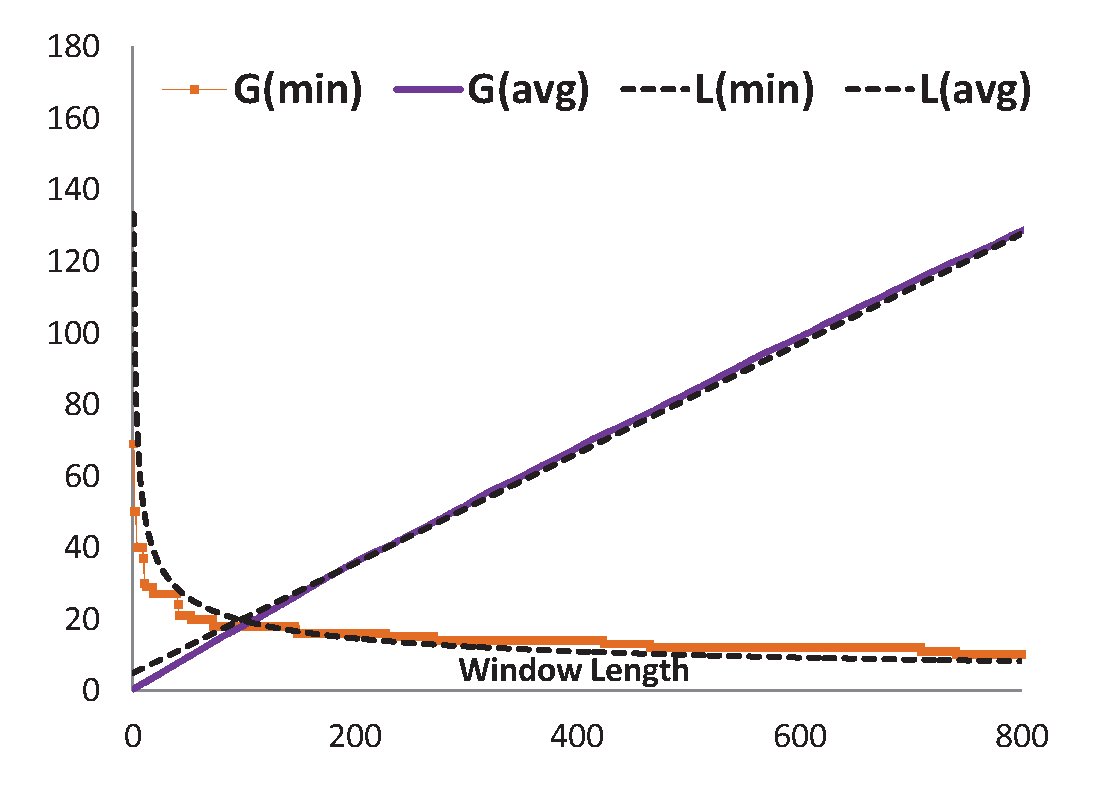
\includegraphics[width=\textwidth]{chapter4/charts/convex.eps}
        \caption{}
%        \label{fig:active_update}
    \end{subfigure}
    \begin{subfigure}[b]{0.45\textwidth}
        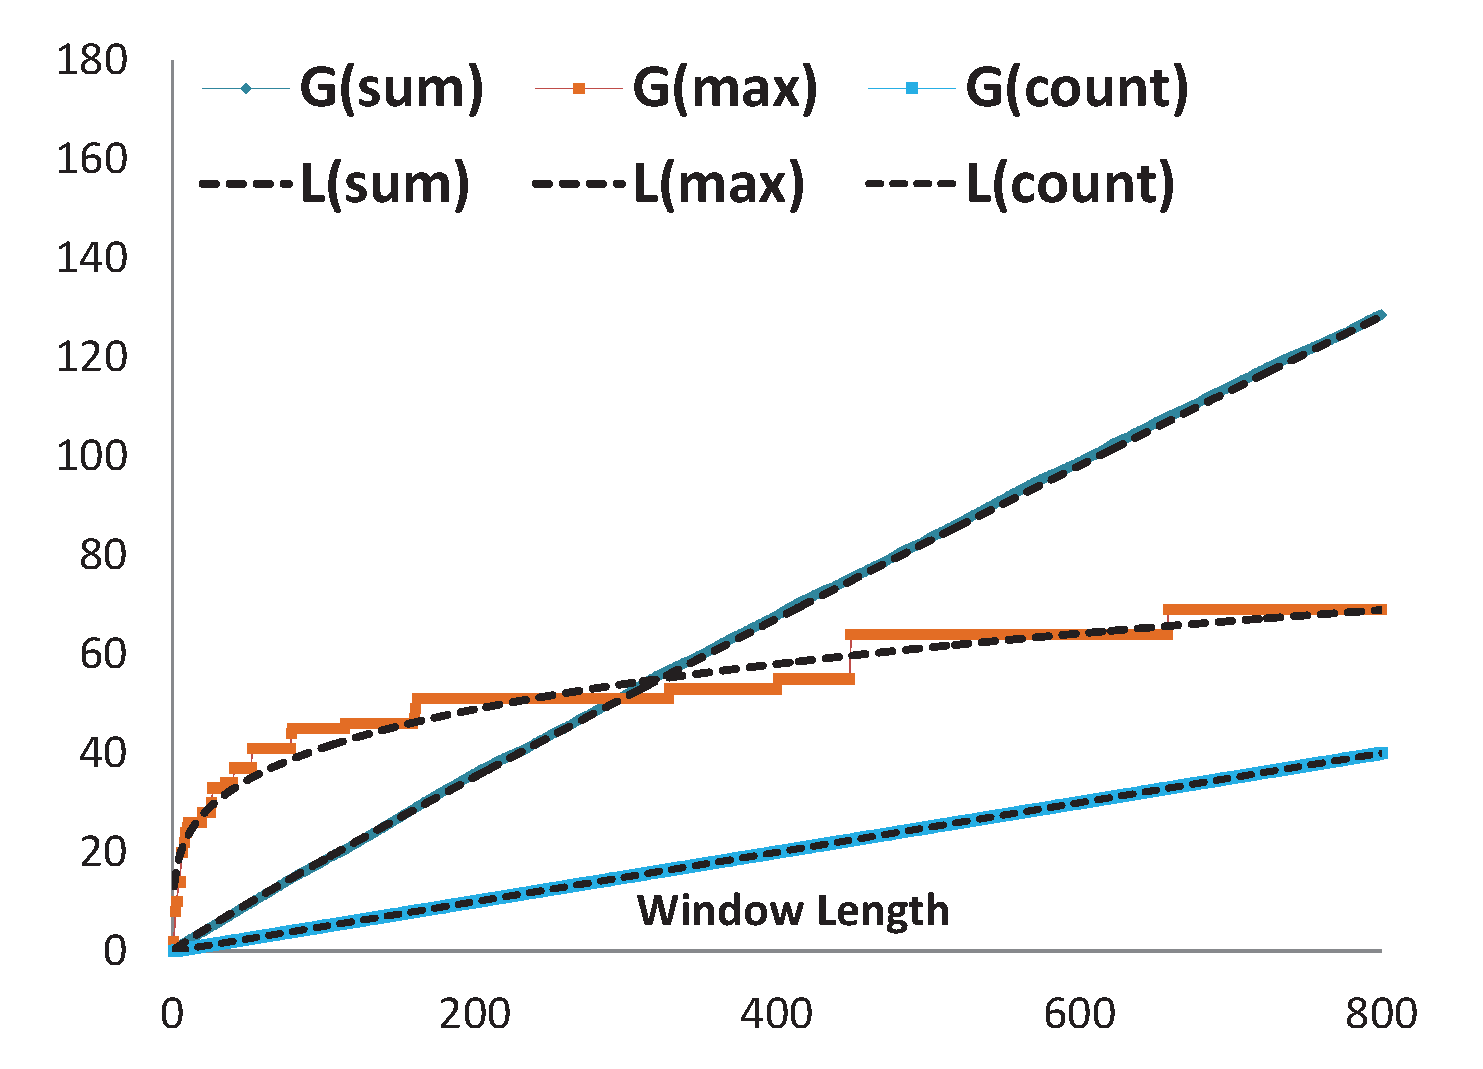
\includegraphics[width=\textwidth]{chapter4/charts/concave.eps}
        \caption{}
%        \label{fig:passive_update}
    \end{subfigure}
    \caption{Illustration of fitting function $L$ on various aggregation functions; solid lines represent $G$ while dotted lines represent $L$. (a) fitting on min and average (b)fitting on max,sum and count.}
    \label{fig:convex_exp}
\end{figure}


\subsubsection{Unseen-window pruning}
\label{sec:useen-window-bound}
Unseen-window pruning utilizes $M_s(w)$ to check if it is necessary to evaluate any 
window $w' \in (w,|\mathbb{H}_s|]$. We observe that $M_s(w)$ can
be efficiently estimated from the values of $J_s(w')$, where $w'\leq w$. 
For example, when $avg$ is used as the aggregate function, $J_s(1)$ is obviously an upper bound for $M_s(w)$ because $J_s(1)$ is essentially the maximum event value. However, such an upper bound is very loose. By utilizing the following theorem, we can derive a tighter bound as follows:

\begin{theorem}[Unseen-Window Bound]
\label{thm:unseen_window_bound}
Given that $J_s(1),$ ..., $J_s(w-1)$ have already been computed, 
%let $M_s = \max\{J_s(t),$ $t\in [w,|\mathbb{H}_s|]\}$,  
%then $M_s$ is estimated as:
let $M_s(w)$ be:
\begin{equation}
M_s(w) = J_s(w) + \min\{\frac{1}{2}J_s(1),\frac{w-1}{w+1}J_s(w-1)\}
\end{equation} 
then $M_s(w)$ is an \emph{unseen-window bound}, i.e. $M_s(w) \geq \max\{J_s(t) | $ $ t\in [w,|\mathbb{H}_s|]\}$
\end{theorem}
\begin{proof}
First, given any integer $k \geq 1$, we see that $J_s(kt) \leq J_s(t)$ 
by making use of Lemma~\ref{lem:subaverage} in a simple induction proof. 
Then, for any integer $x > w$, 
$x$ can be written as $x =\lfloor \frac{x}{w} \rfloor w + x \text{ mod } w$. 
Based on the subadditivity of $J_s(\cdot)$, we have: 
\begin{align*}
J_s(x) &\leq \frac{(\lfloor \frac{x}{w}  \rfloor *w) J_s(\lfloor \frac{x}{w}  \rfloor*w) + (x \text{ mod } w ) J_s(x \text{ mod } w)}{x} \\
&\leq J_s(\lfloor \frac{x}{w}  \rfloor*w) + \frac{x \text{ mod } w}{x} J_s(x \text{ mod } w) \text{, $\lfloor \frac{x}{w}  \rfloor * w \leq x $} \\
&\leq J_s(w) + \frac{x \text{ mod } w}{x} J_s(x \text{ mod } w) \text{, $J_s(kt) \leq J_s(t)$ }
\end{align*}
On one hand, since $t*J_s(t)$ is a monotone increasing function, it follows $(x \text{ mod } w)J_s(x \text{ mod } w) \leq (w-1)J_s(w-1)$. 
Moreover, since $x \geq w+1$, we have $(x \text{ mod } w)\frac{J_s(x \text{ mod } w)}{x}\leq (w-1)\frac{J_s(w-1)}{w+1}$. On the other hand, $J_s(x \text{ mod } w)\leq J_s(1)$ and $\frac{x \text{ mod } w}{x} \leq \frac{1}{2}$ for $x > w$, we have $(x \text{ mod } w)\frac{J_s(x \text{ mod } w)}{x} \leq \frac{1}{2}J_s(1)$.
Then it naturally leads to Theorem~\ref{thm:online_bound}. 
\end{proof}

%The unseen-window bound for other aggregate functions can be derived using similar techniques and 
%the bounds are described in Section~\ref{sec:discussion}.

To utilize $M_s(w)$, after the derivation, we check if $M_s(w)$ is no greater  
than any $\beta(w')$ with $w' >w$,  i.e. $M_s(w) \leq \min\{\beta(w')|w' \in (w ,|\mathbb{H}_s|]\}$. Whenever the condition holds, it is safe to stop further evaluation on subject $s$.
Note that we may maintain an interval tree~\cite{Berg1997Computational} 
on $\beta$ to support efficient checking. 

\begin{theorem}
\label{thm:window_prune}
Each candidate theme returned by Algorithm \ref{algo:prune_overview} has a rank no greater than $p$. 
\end{theorem}
The proof is quite straightforward according to the descriptions for Algorithm~\ref{algo:prune_overview}, visiting-window and unseen-window pruning. Thus, the details are omitted.

\begin{figure}[t]
\centering
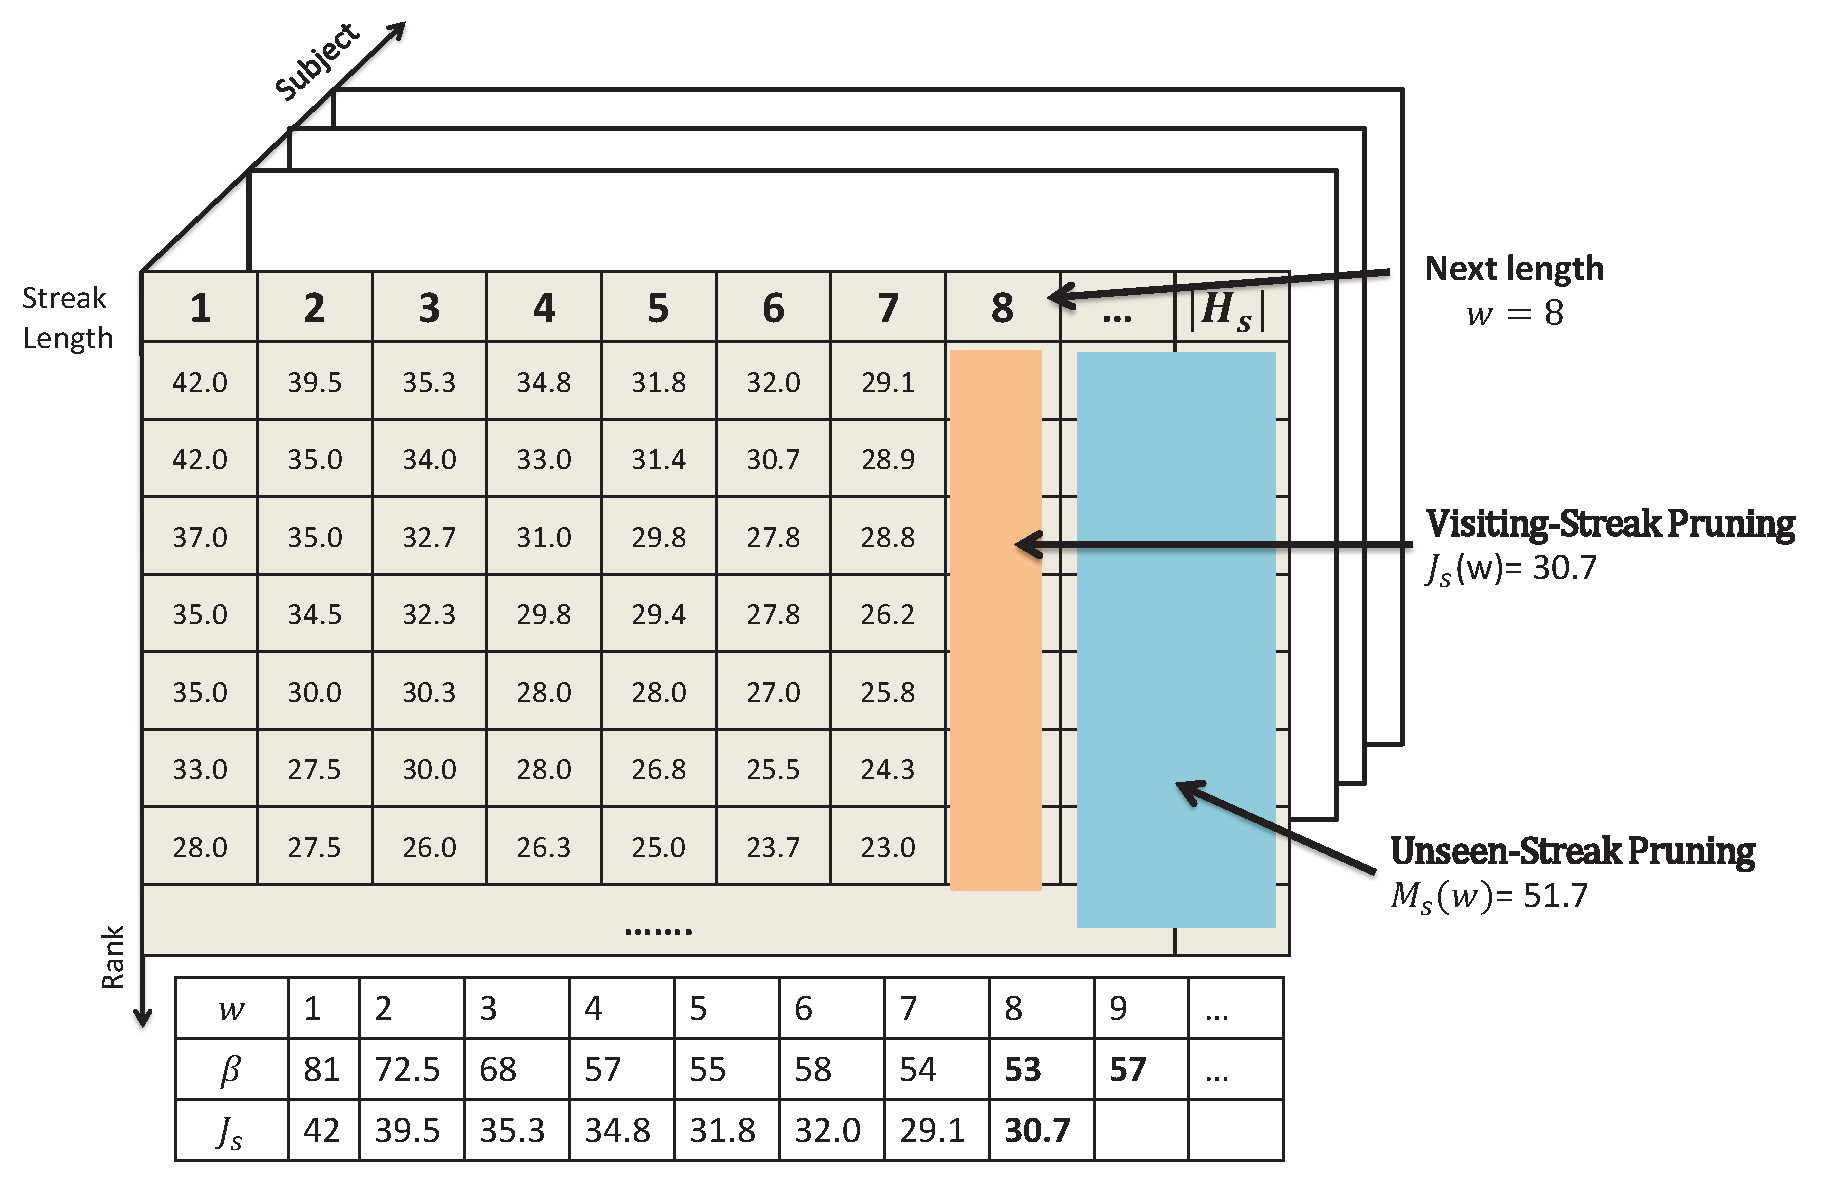
\includegraphics[width=\textwidth]{chapter4/charts/window_pruning.eps}
	\caption{An illustration of window-level pruning techniques. Each square slice represents a
	set of event windows to be computed for a subject, where the column represents window length and the row represents
	the rank. The value in each cell is the aggregate result (i.e., $\overline{v}$) for the corresponding event window.}
\label{fig:window_pruning}
\end{figure}

\begin{example}
We use Fig.~\ref{fig:window_pruning} to illustrate our pruning techniques on a subject $s$.  Each column in the table represents a window length and the cells contain the average values among different event windows with different lengths. For example, the cell in the second row and third column refers to the second largest average value among the event windows with length $3$. Algorithm~\ref{algo:prune_overview} essentially accesses the event windows in increasing order of the window length. Suppose we are about to estimate the upper bound for event windows with length $8$. At this point, the values of $\beta$ and $J_s$ are depicted in the figure. Then, our first job is to estimate the upper bound for all the average values in the $8$-th column.  Based on the values of $J_s(w)$ on smaller windows, we estimate $J_s(8) = \frac{42+7*29.1}{8}= 30.7125$. Since $J_s(8) < \beta(8)$, we can safely prune the whole column, as highlighted in the figure. Afterwards, we estimate the upper bound for all the windows with length larger than $8$. The value of $M_s(8)$ is then estimated as $M_s(8)= 30.7125 + \min\{21, \frac{7}{9}*29.1\}=51.7$. Since all the values of $\beta$ are greater than $M_s(8)$, it is safe to terminate the event window enumeration.
\end{example}

\subsection{Sketch Computation}
After the candidate themes are obtained,
the second step of the sketch discovery process is to, for each subject $s$, extract 
$k$ themes to form sketches $SK_s$ to maximize Eqn.~\ref{eq:scoring_function} (i.e., $g$). 

Our goal of optimizing $g$ is related to the Partly Interval Set Cover (PISC) problem. The goal in PISC is to select a set
of intervals which covers at least a certain percentage of elements. If no rank value is considered in $g$ (i.e., $\alpha = 1$), the
solution in~\cite{golab2009sequential} for PISC maximizes $g$ in $O(\mathbb{H}_s^3)$ time for each subject $s$. However, when
the rank is considered (i.e., $0< \alpha < 1$), optimizing $g$ becomes an open problem as stated in~\cite{edwards2013partial}, where current polynomial time solutions remain unknown.
%
% In PIMC, the ground set contains $n$ points. The input of PIMC is a set of intervals, and a ratio $r$. The goal of PIMC is to find the minimum number
%of intervals which collectively covers at least $rn$ points. The exact methods for solving PIMC takes $O(n^2)$ as stated in~\cite{edwards2013partial}. To use (PIMC) to solve sketch discovery, we may model a candidate theme as an interval, and events of a subject as points.
%Then we may invoke PIMC solution with a $r$ value to find the minimum set of intervals which covers $r\mathbb{H}_s$ events. 
%By examine all possible $r$ values, we are able find the set of intervals maximizing $g$. However, this approach takes $O(\mathbb{H}_s^3)$ time complexity, which is not scalable.
%%NEED TO FURTHER VERIFY
%A related problem to optimizing $g$ is the Partly Interval Max-k Cover problem, where the current best known exact solution~\cite{edwards2013partial} has a quadratic complexity.
To facilitate scalable sketch discovery, we provide 
an efficient $(1-1/e)$ approximation algorithm by exploiting the submodularity property\footnote{A function $I$ is submodular if and only if given two set $A \subseteq B$ and
an element $x \not\in B$, then $I(A \cup \{x\}) - I(A) > I(B \cup \{x\}) - I(B))$.} of the scoring function. Our idea is that since $g$ is not submodular, it is not easy to directly maximize it. However, by applying a relaxation on $g$, we are able
to gain a submodular function $g'$ s.t. maximizing $g'$ would result in
the same optimal solution as maximizing $g$. We design the function of $g'$ as follows:
\begin{equation}
\label{eq:gscore}
g'(\mathbb{X}_s) = \eta_1C'(\mathbb{X}_s) + \eta_2R'(\mathbb{X}_s)
\end{equation}
where $C'(\mathbb{X}_s)$ is the number of distinct events covered by $\mathbb{X}_s$,
 $R'(\mathbb{X}_s) = \Sigma_{X_s \in \mathbb{X}_s}(p-X_s.r)$, $\eta_1 = \alpha/|\mathbb{H}_s|$
and $\eta_2 = (1-\alpha)/k$. Given $k$, $s$ and $g$,
$g'$ is uniquely defined. We have the following theorem which links $g'$ to $g$:

\begin{theorem}
If $A^*$ is the optimal solution wrt. $g'$, then $A^*$ is
also the optimal solution wrt. $g$.
\end{theorem}
\begin{proof}
First observe that, for any set $A \subseteq \mathbb{N}_s$ of size $k$, (i.e., $|A|=k$),
$g(A) = g'(A)$. This can be validated by substituting $A$ into Eq.~\ref{eq:scoring_function} and Eq.~\ref{eq:gscore}. Then,
we prove the theorem by contradiction: 
If $A^*$ is not optimal wrt. $g$, then $\exists B^*$ s.t. $g(B^*) > g(A^*)=g'(A^*)$. However,
since $|B^*|=k$, $g'(B^*)=g(B^*) > g'(A^*)$, which contradicts with $A^*$'s optimality w.r.t. $g'$.
\end{proof}

Henceforth, we are able to compute sketches by maximizing $g'$ instead of $g$. 
We then prove the \emph{submodularity} on $g'$ as stated below:
\begin{theorem}
\label{thm:submodular}
Given a candidate theme set $\mathbb{X}_s$,
$g'(\mathbb{X}_s)$ is submodular.
\end{theorem}
\begin{proof}
Note that $C'$ is a cover function and $R'$ 
is a scalar function, thus $C'$ and $R'$ are both submodular.
Since $g'$ a linear combination of $C'$ and $R'$,
it is also submodular.
%Let $A,B$ be two sets of news candidates with $A\subseteq B$, let $x$ be a news candidate s.t. $x \not\in B$, we have the following according to Eqn.~\ref{eq:gscore}:
%\begin{equation*}
%\begin{split}
% & g'(A \cup \{x\}) - g'(B \cup \{x\})  \\
%& =  \eta_1 C'(A \cup \{x\}) + \eta_2 (R'(A) + R'(\{x\})) \\
%& -  \eta_1 C'(B \cup \{x\}) - \eta_2 (R'(B) + R'(\{x\}) \\
%& = \eta_1 (C(A \cup \{x\}) - C(B \cup \{x\})) +  \eta_2(R'(A) - R'(B)) \\
%& \geq \eta_1(C'(A) - C'(B))+ \eta_2(R'(A) - R'(B)) \text{, $C'$ is submodular}\\
%& = g'(A) - g'(B)
%\end{split}
%\end{equation*}
%Thus, $g'$ is submodular.
\end{proof}

By utilizing the submodularity of $g'$, we apply the greedy algorithm \cite{Fisher1978An} 
to efficiently discover the sketches,
which guarantees a $(1-1/e)$ approximation ratio. 
The greedy sketch discovery scheme is presented in Algorithm~\ref{algo:greedy}. During each step, 
the algorithm picks the best candidate theme which maximizes $g'$ 
among all the candidates which have not been selected yet. The algorithm stops at the $k^{\text{th}}$ iteration.

\begin{algorithm}[h]
\caption{Greedy Sketch Discovery}
\label{algo:greedy}
\begin{algorithmic}[1]
\For {$s \in S$}
\State $\mathbb{N}_s \gets$ candidate themes of subject $s$ filter by Algorithm \ref{algo:prune_overview}
\State $SK_s \gets \{\}$
\For {$t \in [1,k]$}
	\State $x^* \gets \argmax_{x\in \mathbb{N}_s}g'(SK_s\cup \{x\})$ \label{code:greedy}
	\State $SK_s \gets SK_s \cup \{x^*\}$
\EndFor
\EndFor
\State \Return $SK_s \;\; \forall s \in S$
\end{algorithmic}
\end{algorithm}

